% Created by tikzDevice version 0.12 on 2019-03-07 11:10:22
% !TEX encoding = UTF-8 Unicode
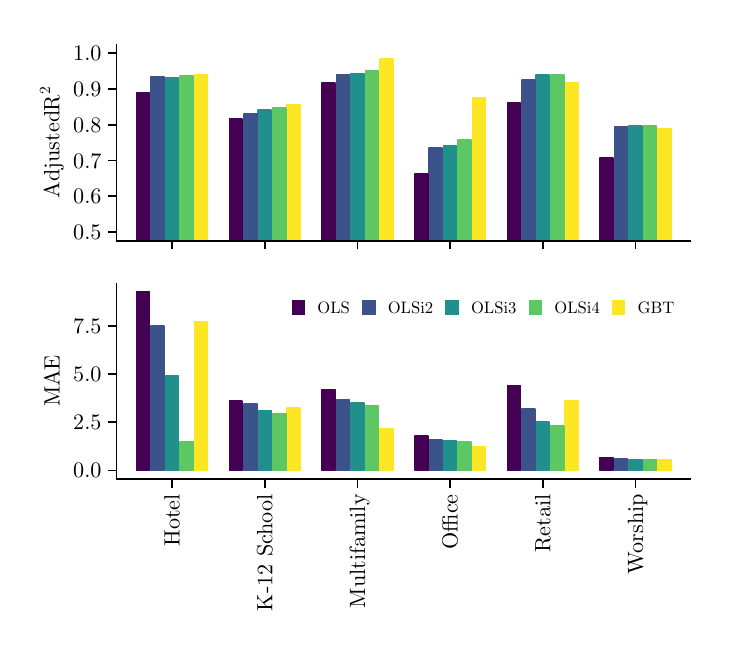
\begin{tikzpicture}[x=1pt,y=1pt]
\definecolor{fillColor}{RGB}{255,255,255}
\path[use as bounding box,fill=fillColor,fill opacity=0.00] (0,0) rectangle (245.72,216.81);
\begin{scope}
\path[clip] (  0.00,130.71) rectangle (245.72,216.81);
\definecolor{drawColor}{RGB}{255,255,255}
\definecolor{fillColor}{RGB}{255,255,255}

\path[draw=drawColor,line width= 0.6pt,line join=round,line cap=round,fill=fillColor] (  0.00,130.71) rectangle (245.72,216.81);
\end{scope}
\begin{scope}
\path[clip] (  0.00,  0.00) rectangle (245.72,130.71);
\definecolor{drawColor}{RGB}{255,255,255}
\definecolor{fillColor}{RGB}{255,255,255}

\path[draw=drawColor,line width= 0.6pt,line join=round,line cap=round,fill=fillColor] (  0.00,  0.00) rectangle (245.72,130.71);
\end{scope}
\begin{scope}
\path[clip] ( 32.07,139.71) rectangle (239.72,210.81);
\definecolor{fillColor}{RGB}{255,255,255}

\path[fill=fillColor] ( 32.07,139.71) rectangle (239.72,210.81);
\definecolor{drawColor}{RGB}{253,231,37}
\definecolor{fillColor}{RGB}{253,231,37}

\path[draw=drawColor,line width= 0.6pt,line join=round,fill=fillColor] ( 60.27, 78.31) rectangle ( 64.96,199.82);
\definecolor{drawColor}{RGB}{93,200,99}
\definecolor{fillColor}{RGB}{93,200,99}

\path[draw=drawColor,line width= 0.6pt,line join=round,fill=fillColor] ( 55.05, 78.31) rectangle ( 59.74,199.43);
\definecolor{drawColor}{RGB}{33,144,140}
\definecolor{fillColor}{RGB}{33,144,140}

\path[draw=drawColor,line width= 0.6pt,line join=round,fill=fillColor] ( 49.82, 78.31) rectangle ( 54.51,198.66);
\definecolor{drawColor}{RGB}{59,82,139}
\definecolor{fillColor}{RGB}{59,82,139}

\path[draw=drawColor,line width= 0.6pt,line join=round,fill=fillColor] ( 44.60, 78.31) rectangle ( 49.29,199.18);
\definecolor{drawColor}{RGB}{68,1,84}
\definecolor{fillColor}{RGB}{68,1,84}

\path[draw=drawColor,line width= 0.6pt,line join=round,fill=fillColor] ( 39.37, 78.31) rectangle ( 44.06,193.10);
\definecolor{drawColor}{RGB}{253,231,37}
\definecolor{fillColor}{RGB}{253,231,37}

\path[draw=drawColor,line width= 0.6pt,line join=round,fill=fillColor] ( 93.76, 78.31) rectangle ( 98.45,189.09);
\definecolor{drawColor}{RGB}{93,200,99}
\definecolor{fillColor}{RGB}{93,200,99}

\path[draw=drawColor,line width= 0.6pt,line join=round,fill=fillColor] ( 88.54, 78.31) rectangle ( 93.23,187.80);
\definecolor{drawColor}{RGB}{33,144,140}
\definecolor{fillColor}{RGB}{33,144,140}

\path[draw=drawColor,line width= 0.6pt,line join=round,fill=fillColor] ( 83.31, 78.31) rectangle ( 88.00,187.02);
\definecolor{drawColor}{RGB}{59,82,139}
\definecolor{fillColor}{RGB}{59,82,139}

\path[draw=drawColor,line width= 0.6pt,line join=round,fill=fillColor] ( 78.09, 78.31) rectangle ( 82.78,185.73);
\definecolor{drawColor}{RGB}{68,1,84}
\definecolor{fillColor}{RGB}{68,1,84}

\path[draw=drawColor,line width= 0.6pt,line join=round,fill=fillColor] ( 72.87, 78.31) rectangle ( 77.55,183.92);
\definecolor{drawColor}{RGB}{253,231,37}
\definecolor{fillColor}{RGB}{253,231,37}

\path[draw=drawColor,line width= 0.6pt,line join=round,fill=fillColor] (127.26, 78.31) rectangle (131.94,205.51);
\definecolor{drawColor}{RGB}{93,200,99}
\definecolor{fillColor}{RGB}{93,200,99}

\path[draw=drawColor,line width= 0.6pt,line join=round,fill=fillColor] (122.03, 78.31) rectangle (126.72,201.24);
\definecolor{drawColor}{RGB}{33,144,140}
\definecolor{fillColor}{RGB}{33,144,140}

\path[draw=drawColor,line width= 0.6pt,line join=round,fill=fillColor] (116.81, 78.31) rectangle (121.49,200.21);
\definecolor{drawColor}{RGB}{59,82,139}
\definecolor{fillColor}{RGB}{59,82,139}

\path[draw=drawColor,line width= 0.6pt,line join=round,fill=fillColor] (111.58, 78.31) rectangle (116.27,199.82);
\definecolor{drawColor}{RGB}{68,1,84}
\definecolor{fillColor}{RGB}{68,1,84}

\path[draw=drawColor,line width= 0.6pt,line join=round,fill=fillColor] (106.36, 78.31) rectangle (111.05,196.85);
\definecolor{drawColor}{RGB}{253,231,37}
\definecolor{fillColor}{RGB}{253,231,37}

\path[draw=drawColor,line width= 0.6pt,line join=round,fill=fillColor] (160.75, 78.31) rectangle (165.43,191.42);
\definecolor{drawColor}{RGB}{93,200,99}
\definecolor{fillColor}{RGB}{93,200,99}

\path[draw=drawColor,line width= 0.6pt,line join=round,fill=fillColor] (155.52, 78.31) rectangle (160.21,176.29);
\definecolor{drawColor}{RGB}{33,144,140}
\definecolor{fillColor}{RGB}{33,144,140}

\path[draw=drawColor,line width= 0.6pt,line join=round,fill=fillColor] (150.30, 78.31) rectangle (154.99,174.23);
\definecolor{drawColor}{RGB}{59,82,139}
\definecolor{fillColor}{RGB}{59,82,139}

\path[draw=drawColor,line width= 0.6pt,line join=round,fill=fillColor] (145.07, 78.31) rectangle (149.76,173.32);
\definecolor{drawColor}{RGB}{68,1,84}
\definecolor{fillColor}{RGB}{68,1,84}

\path[draw=drawColor,line width= 0.6pt,line join=round,fill=fillColor] (139.85, 78.31) rectangle (144.54,163.88);
\definecolor{drawColor}{RGB}{253,231,37}
\definecolor{fillColor}{RGB}{253,231,37}

\path[draw=drawColor,line width= 0.6pt,line join=round,fill=fillColor] (194.24, 78.31) rectangle (198.93,196.98);
\definecolor{drawColor}{RGB}{93,200,99}
\definecolor{fillColor}{RGB}{93,200,99}

\path[draw=drawColor,line width= 0.6pt,line join=round,fill=fillColor] (189.01, 78.31) rectangle (193.70,199.82);
\definecolor{drawColor}{RGB}{33,144,140}
\definecolor{fillColor}{RGB}{33,144,140}

\path[draw=drawColor,line width= 0.6pt,line join=round,fill=fillColor] (183.79, 78.31) rectangle (188.48,199.69);
\definecolor{drawColor}{RGB}{59,82,139}
\definecolor{fillColor}{RGB}{59,82,139}

\path[draw=drawColor,line width= 0.6pt,line join=round,fill=fillColor] (178.56, 78.31) rectangle (183.25,197.88);
\definecolor{drawColor}{RGB}{68,1,84}
\definecolor{fillColor}{RGB}{68,1,84}

\path[draw=drawColor,line width= 0.6pt,line join=round,fill=fillColor] (173.34, 78.31) rectangle (178.03,189.48);
\definecolor{drawColor}{RGB}{253,231,37}
\definecolor{fillColor}{RGB}{253,231,37}

\path[draw=drawColor,line width= 0.6pt,line join=round,fill=fillColor] (227.73, 78.31) rectangle (232.42,180.43);
\definecolor{drawColor}{RGB}{93,200,99}
\definecolor{fillColor}{RGB}{93,200,99}

\path[draw=drawColor,line width= 0.6pt,line join=round,fill=fillColor] (222.50, 78.31) rectangle (227.19,181.34);
\definecolor{drawColor}{RGB}{33,144,140}
\definecolor{fillColor}{RGB}{33,144,140}

\path[draw=drawColor,line width= 0.6pt,line join=round,fill=fillColor] (217.28, 78.31) rectangle (221.97,181.34);
\definecolor{drawColor}{RGB}{59,82,139}
\definecolor{fillColor}{RGB}{59,82,139}

\path[draw=drawColor,line width= 0.6pt,line join=round,fill=fillColor] (212.05, 78.31) rectangle (216.74,180.82);
\definecolor{drawColor}{RGB}{68,1,84}
\definecolor{fillColor}{RGB}{68,1,84}

\path[draw=drawColor,line width= 0.6pt,line join=round,fill=fillColor] (206.83, 78.31) rectangle (211.52,169.83);
\end{scope}
\begin{scope}
\path[clip] ( 32.07, 53.61) rectangle (239.72,124.71);
\definecolor{fillColor}{RGB}{255,255,255}

\path[fill=fillColor] ( 32.07, 53.61) rectangle (239.72,124.71);
\definecolor{drawColor}{RGB}{253,231,37}
\definecolor{fillColor}{RGB}{253,231,37}

\path[draw=drawColor,line width= 0.6pt,line join=round,fill=fillColor] ( 60.27, 56.84) rectangle ( 64.96,110.50);
\definecolor{drawColor}{RGB}{93,200,99}
\definecolor{fillColor}{RGB}{93,200,99}

\path[draw=drawColor,line width= 0.6pt,line join=round,fill=fillColor] ( 55.05, 56.84) rectangle ( 59.74, 67.27);
\definecolor{drawColor}{RGB}{33,144,140}
\definecolor{fillColor}{RGB}{33,144,140}

\path[draw=drawColor,line width= 0.6pt,line join=round,fill=fillColor] ( 49.82, 56.84) rectangle ( 54.51, 91.04);
\definecolor{drawColor}{RGB}{59,82,139}
\definecolor{fillColor}{RGB}{59,82,139}

\path[draw=drawColor,line width= 0.6pt,line join=round,fill=fillColor] ( 44.60, 56.84) rectangle ( 49.29,108.90);
\definecolor{drawColor}{RGB}{68,1,84}
\definecolor{fillColor}{RGB}{68,1,84}

\path[draw=drawColor,line width= 0.6pt,line join=round,fill=fillColor] ( 39.37, 56.84) rectangle ( 44.06,121.48);
\definecolor{drawColor}{RGB}{253,231,37}
\definecolor{fillColor}{RGB}{253,231,37}

\path[draw=drawColor,line width= 0.6pt,line join=round,fill=fillColor] ( 93.76, 56.84) rectangle ( 98.45, 79.36);
\definecolor{drawColor}{RGB}{93,200,99}
\definecolor{fillColor}{RGB}{93,200,99}

\path[draw=drawColor,line width= 0.6pt,line join=round,fill=fillColor] ( 88.54, 56.84) rectangle ( 93.23, 77.35);
\definecolor{drawColor}{RGB}{33,144,140}
\definecolor{fillColor}{RGB}{33,144,140}

\path[draw=drawColor,line width= 0.6pt,line join=round,fill=fillColor] ( 83.31, 56.84) rectangle ( 88.00, 78.53);
\definecolor{drawColor}{RGB}{59,82,139}
\definecolor{fillColor}{RGB}{59,82,139}

\path[draw=drawColor,line width= 0.6pt,line join=round,fill=fillColor] ( 78.09, 56.84) rectangle ( 82.78, 80.89);
\definecolor{drawColor}{RGB}{68,1,84}
\definecolor{fillColor}{RGB}{68,1,84}

\path[draw=drawColor,line width= 0.6pt,line join=round,fill=fillColor] ( 72.87, 56.84) rectangle ( 77.55, 81.79);
\definecolor{drawColor}{RGB}{253,231,37}
\definecolor{fillColor}{RGB}{253,231,37}

\path[draw=drawColor,line width= 0.6pt,line join=round,fill=fillColor] (127.26, 56.84) rectangle (131.94, 71.79);
\definecolor{drawColor}{RGB}{93,200,99}
\definecolor{fillColor}{RGB}{93,200,99}

\path[draw=drawColor,line width= 0.6pt,line join=round,fill=fillColor] (122.03, 56.84) rectangle (126.72, 80.06);
\definecolor{drawColor}{RGB}{33,144,140}
\definecolor{fillColor}{RGB}{33,144,140}

\path[draw=drawColor,line width= 0.6pt,line join=round,fill=fillColor] (116.81, 56.84) rectangle (121.49, 81.24);
\definecolor{drawColor}{RGB}{59,82,139}
\definecolor{fillColor}{RGB}{59,82,139}

\path[draw=drawColor,line width= 0.6pt,line join=round,fill=fillColor] (111.58, 56.84) rectangle (116.27, 82.35);
\definecolor{drawColor}{RGB}{68,1,84}
\definecolor{fillColor}{RGB}{68,1,84}

\path[draw=drawColor,line width= 0.6pt,line join=round,fill=fillColor] (106.36, 56.84) rectangle (111.05, 86.03);
\definecolor{drawColor}{RGB}{253,231,37}
\definecolor{fillColor}{RGB}{253,231,37}

\path[draw=drawColor,line width= 0.6pt,line join=round,fill=fillColor] (160.75, 56.84) rectangle (165.43, 65.25);
\definecolor{drawColor}{RGB}{93,200,99}
\definecolor{fillColor}{RGB}{93,200,99}

\path[draw=drawColor,line width= 0.6pt,line join=round,fill=fillColor] (155.52, 56.84) rectangle (160.21, 67.06);
\definecolor{drawColor}{RGB}{33,144,140}
\definecolor{fillColor}{RGB}{33,144,140}

\path[draw=drawColor,line width= 0.6pt,line join=round,fill=fillColor] (150.30, 56.84) rectangle (154.99, 67.62);
\definecolor{drawColor}{RGB}{59,82,139}
\definecolor{fillColor}{RGB}{59,82,139}

\path[draw=drawColor,line width= 0.6pt,line join=round,fill=fillColor] (145.07, 56.84) rectangle (149.76, 67.76);
\definecolor{drawColor}{RGB}{68,1,84}
\definecolor{fillColor}{RGB}{68,1,84}

\path[draw=drawColor,line width= 0.6pt,line join=round,fill=fillColor] (139.85, 56.84) rectangle (144.54, 69.35);
\definecolor{drawColor}{RGB}{253,231,37}
\definecolor{fillColor}{RGB}{253,231,37}

\path[draw=drawColor,line width= 0.6pt,line join=round,fill=fillColor] (194.24, 56.84) rectangle (198.93, 81.93);
\definecolor{drawColor}{RGB}{93,200,99}
\definecolor{fillColor}{RGB}{93,200,99}

\path[draw=drawColor,line width= 0.6pt,line join=round,fill=fillColor] (189.01, 56.84) rectangle (193.70, 72.83);
\definecolor{drawColor}{RGB}{33,144,140}
\definecolor{fillColor}{RGB}{33,144,140}

\path[draw=drawColor,line width= 0.6pt,line join=round,fill=fillColor] (183.79, 56.84) rectangle (188.48, 74.29);
\definecolor{drawColor}{RGB}{59,82,139}
\definecolor{fillColor}{RGB}{59,82,139}

\path[draw=drawColor,line width= 0.6pt,line join=round,fill=fillColor] (178.56, 56.84) rectangle (183.25, 78.94);
\definecolor{drawColor}{RGB}{68,1,84}
\definecolor{fillColor}{RGB}{68,1,84}

\path[draw=drawColor,line width= 0.6pt,line join=round,fill=fillColor] (173.34, 56.84) rectangle (178.03, 87.56);
\definecolor{drawColor}{RGB}{253,231,37}
\definecolor{fillColor}{RGB}{253,231,37}

\path[draw=drawColor,line width= 0.6pt,line join=round,fill=fillColor] (227.73, 56.84) rectangle (232.42, 60.74);
\definecolor{drawColor}{RGB}{93,200,99}
\definecolor{fillColor}{RGB}{93,200,99}

\path[draw=drawColor,line width= 0.6pt,line join=round,fill=fillColor] (222.50, 56.84) rectangle (227.19, 60.74);
\definecolor{drawColor}{RGB}{33,144,140}
\definecolor{fillColor}{RGB}{33,144,140}

\path[draw=drawColor,line width= 0.6pt,line join=round,fill=fillColor] (217.28, 56.84) rectangle (221.97, 60.81);
\definecolor{drawColor}{RGB}{59,82,139}
\definecolor{fillColor}{RGB}{59,82,139}

\path[draw=drawColor,line width= 0.6pt,line join=round,fill=fillColor] (212.05, 56.84) rectangle (216.74, 60.87);
\definecolor{drawColor}{RGB}{68,1,84}
\definecolor{fillColor}{RGB}{68,1,84}

\path[draw=drawColor,line width= 0.6pt,line join=round,fill=fillColor] (206.83, 56.84) rectangle (211.52, 61.43);
\end{scope}
\begin{scope}
\path[clip] (  0.00,  0.00) rectangle (245.72,216.81);
\definecolor{drawColor}{RGB}{0,0,0}

\path[draw=drawColor,line width= 0.6pt,line join=round] ( 32.07,139.71) --
	( 32.07,210.81);
\end{scope}
\begin{scope}
\path[clip] (  0.00,  0.00) rectangle (245.72,216.81);
\definecolor{drawColor}{RGB}{0,0,0}

\node[text=drawColor,anchor=base east,inner sep=0pt, outer sep=0pt, scale=  0.80] at ( 26.67,140.19) {0.5};

\node[text=drawColor,anchor=base east,inner sep=0pt, outer sep=0pt, scale=  0.80] at ( 26.67,153.12) {0.6};

\node[text=drawColor,anchor=base east,inner sep=0pt, outer sep=0pt, scale=  0.80] at ( 26.67,166.04) {0.7};

\node[text=drawColor,anchor=base east,inner sep=0pt, outer sep=0pt, scale=  0.80] at ( 26.67,178.97) {0.8};

\node[text=drawColor,anchor=base east,inner sep=0pt, outer sep=0pt, scale=  0.80] at ( 26.67,191.90) {0.9};

\node[text=drawColor,anchor=base east,inner sep=0pt, outer sep=0pt, scale=  0.80] at ( 26.67,204.82) {1.0};
\end{scope}
\begin{scope}
\path[clip] (  0.00,  0.00) rectangle (245.72,216.81);
\definecolor{drawColor}{RGB}{0,0,0}

\path[draw=drawColor,line width= 0.6pt,line join=round] ( 29.07,142.94) --
	( 32.07,142.94);

\path[draw=drawColor,line width= 0.6pt,line join=round] ( 29.07,155.87) --
	( 32.07,155.87);

\path[draw=drawColor,line width= 0.6pt,line join=round] ( 29.07,168.80) --
	( 32.07,168.80);

\path[draw=drawColor,line width= 0.6pt,line join=round] ( 29.07,181.72) --
	( 32.07,181.72);

\path[draw=drawColor,line width= 0.6pt,line join=round] ( 29.07,194.65) --
	( 32.07,194.65);

\path[draw=drawColor,line width= 0.6pt,line join=round] ( 29.07,207.58) --
	( 32.07,207.58);
\end{scope}
\begin{scope}
\path[clip] (  0.00,  0.00) rectangle (245.72,216.81);
\definecolor{drawColor}{RGB}{0,0,0}

\path[draw=drawColor,line width= 0.6pt,line join=round] ( 32.07, 53.61) --
	( 32.07,124.71);
\end{scope}
\begin{scope}
\path[clip] (  0.00,  0.00) rectangle (245.72,216.81);
\definecolor{drawColor}{RGB}{0,0,0}

\node[text=drawColor,anchor=base east,inner sep=0pt, outer sep=0pt, scale=  0.80] at ( 26.67, 54.09) {0.0};

\node[text=drawColor,anchor=base east,inner sep=0pt, outer sep=0pt, scale=  0.80] at ( 26.67, 71.46) {2.5};

\node[text=drawColor,anchor=base east,inner sep=0pt, outer sep=0pt, scale=  0.80] at ( 26.67, 88.84) {5.0};

\node[text=drawColor,anchor=base east,inner sep=0pt, outer sep=0pt, scale=  0.80] at ( 26.67,106.21) {7.5};
\end{scope}
\begin{scope}
\path[clip] (  0.00,  0.00) rectangle (245.72,216.81);
\definecolor{drawColor}{RGB}{0,0,0}

\path[draw=drawColor,line width= 0.6pt,line join=round] ( 29.07, 56.84) --
	( 32.07, 56.84);

\path[draw=drawColor,line width= 0.6pt,line join=round] ( 29.07, 74.22) --
	( 32.07, 74.22);

\path[draw=drawColor,line width= 0.6pt,line join=round] ( 29.07, 91.59) --
	( 32.07, 91.59);

\path[draw=drawColor,line width= 0.6pt,line join=round] ( 29.07,108.97) --
	( 32.07,108.97);
\end{scope}
\begin{scope}
\path[clip] (  0.00,  0.00) rectangle (245.72,216.81);
\definecolor{drawColor}{RGB}{0,0,0}

\path[draw=drawColor,line width= 0.6pt,line join=round] ( 32.07,139.71) --
	(239.72,139.71);
\end{scope}
\begin{scope}
\path[clip] (  0.00,  0.00) rectangle (245.72,216.81);
\definecolor{drawColor}{RGB}{0,0,0}

\path[draw=drawColor,line width= 0.6pt,line join=round] ( 52.17,136.71) --
	( 52.17,139.71);

\path[draw=drawColor,line width= 0.6pt,line join=round] ( 85.66,136.71) --
	( 85.66,139.71);

\path[draw=drawColor,line width= 0.6pt,line join=round] (119.15,136.71) --
	(119.15,139.71);

\path[draw=drawColor,line width= 0.6pt,line join=round] (152.64,136.71) --
	(152.64,139.71);

\path[draw=drawColor,line width= 0.6pt,line join=round] (186.13,136.71) --
	(186.13,139.71);

\path[draw=drawColor,line width= 0.6pt,line join=round] (219.62,136.71) --
	(219.62,139.71);
\end{scope}
\begin{scope}
\path[clip] (  0.00,  0.00) rectangle (245.72,216.81);
\definecolor{drawColor}{RGB}{0,0,0}

\path[draw=drawColor,line width= 0.6pt,line join=round] ( 32.07, 53.61) --
	(239.72, 53.61);
\end{scope}
\begin{scope}
\path[clip] (  0.00,  0.00) rectangle (245.72,216.81);
\definecolor{drawColor}{RGB}{0,0,0}

\path[draw=drawColor,line width= 0.6pt,line join=round] ( 52.17, 50.61) --
	( 52.17, 53.61);

\path[draw=drawColor,line width= 0.6pt,line join=round] ( 85.66, 50.61) --
	( 85.66, 53.61);

\path[draw=drawColor,line width= 0.6pt,line join=round] (119.15, 50.61) --
	(119.15, 53.61);

\path[draw=drawColor,line width= 0.6pt,line join=round] (152.64, 50.61) --
	(152.64, 53.61);

\path[draw=drawColor,line width= 0.6pt,line join=round] (186.13, 50.61) --
	(186.13, 53.61);

\path[draw=drawColor,line width= 0.6pt,line join=round] (219.62, 50.61) --
	(219.62, 53.61);
\end{scope}
\begin{scope}
\path[clip] (  0.00,  0.00) rectangle (245.72,216.81);
\definecolor{drawColor}{RGB}{0,0,0}

\node[text=drawColor,rotate= 90.00,anchor=base east,inner sep=0pt, outer sep=0pt, scale=  0.80] at ( 54.92, 48.21) {Hotel};

\node[text=drawColor,rotate= 90.00,anchor=base east,inner sep=0pt, outer sep=0pt, scale=  0.80] at ( 88.41, 48.21) {K-12 School};

\node[text=drawColor,rotate= 90.00,anchor=base east,inner sep=0pt, outer sep=0pt, scale=  0.80] at (121.91, 48.21) {Multifamily};

\node[text=drawColor,rotate= 90.00,anchor=base east,inner sep=0pt, outer sep=0pt, scale=  0.80] at (155.40, 48.21) {Office};

\node[text=drawColor,rotate= 90.00,anchor=base east,inner sep=0pt, outer sep=0pt, scale=  0.80] at (188.89, 48.21) {Retail};

\node[text=drawColor,rotate= 90.00,anchor=base east,inner sep=0pt, outer sep=0pt, scale=  0.80] at (222.38, 48.21) {Worship};
\end{scope}
\begin{scope}
\path[clip] (  0.00,  0.00) rectangle (245.72,216.81);
\definecolor{drawColor}{RGB}{0,0,0}

\node[text=drawColor,rotate= 90.00,anchor=base west,inner sep=0pt, outer sep=0pt, scale=  0.80] at ( 11.41,155.23) {Adjusted };

\node[text=drawColor,rotate= 90.00,anchor=base west,inner sep=0pt, outer sep=0pt, scale=  0.80] at ( 11.41,186.60) {R};

\node[text=drawColor,rotate= 90.00,anchor=base west,inner sep=0pt, outer sep=0pt, scale=  0.56] at (  8.14,192.49) {2};
\end{scope}
\begin{scope}
\path[clip] (  0.00,  0.00) rectangle (245.72,216.81);
\definecolor{drawColor}{RGB}{0,0,0}

\node[text=drawColor,rotate= 90.00,anchor=base west,inner sep=0pt, outer sep=0pt, scale=  0.80] at ( 11.51, 79.77) {MAE};
\end{scope}
\begin{scope}
\path[clip] (  0.00,  0.00) rectangle (245.72,216.81);
\definecolor{fillColor}{RGB}{255,255,255}

\path[fill=fillColor] ( 84.99,105.26) rectangle (239.72,124.71);
\end{scope}
\begin{scope}
\path[clip] (  0.00,  0.00) rectangle (245.72,216.81);
\definecolor{drawColor}{RGB}{68,1,84}
\definecolor{fillColor}{RGB}{68,1,84}

\path[draw=drawColor,line width= 0.6pt,line cap=round,fill=fillColor] ( 95.70,113.35) rectangle ( 99.97,118.00);
\end{scope}
\begin{scope}
\path[clip] (  0.00,  0.00) rectangle (245.72,216.81);
\definecolor{drawColor}{RGB}{59,82,139}
\definecolor{fillColor}{RGB}{59,82,139}

\path[draw=drawColor,line width= 0.6pt,line cap=round,fill=fillColor] (121.14,113.35) rectangle (125.41,118.00);
\end{scope}
\begin{scope}
\path[clip] (  0.00,  0.00) rectangle (245.72,216.81);
\definecolor{drawColor}{RGB}{33,144,140}
\definecolor{fillColor}{RGB}{33,144,140}

\path[draw=drawColor,line width= 0.6pt,line cap=round,fill=fillColor] (151.24,113.35) rectangle (155.51,118.00);
\end{scope}
\begin{scope}
\path[clip] (  0.00,  0.00) rectangle (245.72,216.81);
\definecolor{drawColor}{RGB}{93,200,99}
\definecolor{fillColor}{RGB}{93,200,99}

\path[draw=drawColor,line width= 0.6pt,line cap=round,fill=fillColor] (181.35,113.35) rectangle (185.61,118.00);
\end{scope}
\begin{scope}
\path[clip] (  0.00,  0.00) rectangle (245.72,216.81);
\definecolor{drawColor}{RGB}{253,231,37}
\definecolor{fillColor}{RGB}{253,231,37}

\path[draw=drawColor,line width= 0.6pt,line cap=round,fill=fillColor] (211.45,113.35) rectangle (215.72,118.00);
\end{scope}
\begin{scope}
\path[clip] (  0.00,  0.00) rectangle (245.72,216.81);
\definecolor{drawColor}{RGB}{0,0,0}

\node[text=drawColor,anchor=base west,inner sep=0pt, outer sep=0pt, scale=  0.60] at (104.68,113.61) {OLS};
\end{scope}
\begin{scope}
\path[clip] (  0.00,  0.00) rectangle (245.72,216.81);
\definecolor{drawColor}{RGB}{0,0,0}

\node[text=drawColor,anchor=base west,inner sep=0pt, outer sep=0pt, scale=  0.60] at (130.12,113.61) {OLSi2};
\end{scope}
\begin{scope}
\path[clip] (  0.00,  0.00) rectangle (245.72,216.81);
\definecolor{drawColor}{RGB}{0,0,0}

\node[text=drawColor,anchor=base west,inner sep=0pt, outer sep=0pt, scale=  0.60] at (160.22,113.61) {OLSi3};
\end{scope}
\begin{scope}
\path[clip] (  0.00,  0.00) rectangle (245.72,216.81);
\definecolor{drawColor}{RGB}{0,0,0}

\node[text=drawColor,anchor=base west,inner sep=0pt, outer sep=0pt, scale=  0.60] at (190.33,113.61) {OLSi4};
\end{scope}
\begin{scope}
\path[clip] (  0.00,  0.00) rectangle (245.72,216.81);
\definecolor{drawColor}{RGB}{0,0,0}

\node[text=drawColor,anchor=base west,inner sep=0pt, outer sep=0pt, scale=  0.60] at (220.43,113.61) {GBT};
\end{scope}
\end{tikzpicture}
